\documentclass[main.tex]{subfiles}
\begin{document}
\chapter{Introduction}

\epigraph{In the beginning the Universe was created. This has made a lot of people very angry and been widely regarded as a bad move.}{Douglas Adams}

Welcome! This book is essentially my own typed-up notes/explanations from the \textit{Discrete Structures} (CMSC250) course at UMD. There may be typos -- my apologies. My hope is to improve your overall understanding of the course content. If you're willing to put forth the effort to \textit{understand} the course material, and think mathematically, then you will succeed.

\section{What is Discrete Mathematics?}

Sometimes the actual name of the course is never addressed in-class. The `mathematics' part hopefully should be familiar -- numbers and stuff. What does `discrete' mean? Well, Merriam-Webster provides two good definitions:

\begin{defn}[Discrete\index{Discrete}]
	\leavevmode
	\begin{itemize}
		\item consisting of distinct or unconnected elements
		\item taking on or having a finite or countably infinite number of values
	\end{itemize}
\end{defn}

Consider the real number line:

\begin{center}
\begin{tikzpicture}
\draw[latex-] (-6.5,0) -- (6.5,0) ;
\draw[-latex] (-6.5,0) -- (6.5,0) ;
\foreach \x in  {-6,-4,-2,0,2,4,6}
\draw[shift={(\x,0)},color=black] (0pt,3pt) -- (0pt,-3pt);
\foreach \x in {-6,-4,-2,0,2,4,6}
\draw[shift={(\x,0)},color=black] (0pt,0pt) -- (0pt,-3pt) node[below] 
{$\x$};
\fill (3.14159,0) circle[radius=2pt];
\end{tikzpicture}
\end{center}

We can point to any position on the line and find some real number to represent that point. It may have some long string of decimal digits, however we can do it. In the example above, the point is \(\pi \approx 3.14159\). We refer to this real line as \textit{continuous}\index{Continuous}. Broken up in-between all of these real numbers is a set of discrete points \(\{\cdots,-2,-1,0,1,2,\cdots\}\). These points are not continuous, and hence discrete, since we must make a jump (on the real line) from number to number. Our goal in this class is to examine these discrete numbers (which we call the \textit{Integers} \(\Z\)) and structures.

\section{Why Should You Care?}

It seems somewhat pointless just to learn this whole proof crap (that you figured you never had to do again -- see high school Geometry) when you will probably never use it again. So, here (in no particular order) is a list of reasons for and against learning this material.

\begin{multicols}{2}
	\begin{center}
		\textsc{for}
	\end{center}
	\begin{itemize}
		\item You become a free-thinker, and you become more skeptical
		\item You begin to question your world and your own perceptions
		\item The mathematical mindset will help you throughout your life, and will be especially useful while coding
		\item Your creativity comes back, and you may end up enjoying the course
		\item Computer science is just applied mathematics
	\end{itemize}
	
	\columnbreak
	
	\begin{center}
		\textsc{against}
	\end{center}
	\begin{itemize}
		\item Proofs are boring and math sucks
		\item Other people can do the proofs and math for me -- I am willing to accept their work
		\item Discrete math is just a weed-out class
		\item I do not need math to know how to code
		\item Discrete math will not improve my programming
	\end{itemize}
\end{multicols}

If you disagree with any of the \textsc{for} reasons, then you should strongly consider why you chose computer science. We now provide counter-arguments to each of the above \textsc{against} points.

First, proofs and math are very akin to problem-solving. Programming is entirely problem-solving. If you do not enjoy problem-solving, then you are going to hate any programming job you get and you should really consider why you chose computer science.

Second, having other people do the leg-work will only get you so far in life. Eventually, someone is going to ask you to do the hard part too. Plus, if you blindly accept other people's work without checking it for yourself, you become vulnerable to mistakes. Unchecked work leads to mistakes, which leads to wasted money and lost revenue, which leads to you getting fired from your job.

Third, discrete math is a weed-out class in the sense of the previous point. It is a basis for computer science, and if you do poorly in it then that may be an indicator of your future success in the field.

Fourth, yeah right.

Fifth, you keep telling yourself that while the top programmers at Google use mathematical reasoning to create super-fast mapping algorithms.

\section{An Exercise in Proof}

Maybe you are not convinced that proof is useful and necessary. Well, consider the following problem.

\begin{boxx}
	Draw a circle and place \(n\) points on the edge of the circle. Draw a line between each possible pair of points. This will yield closed regions within the circle. How many such regions are there for \(n \geq 1\) points?
\end{boxx}

Try it for \(n = 1,2,3,4,5\). We will ignore \(n=0\) for this exercise. You should get:

\begin{center}
	\begin{tabular}{c|ccccc}
		\(n\) & 1 & 2 & 3 & 4 & 5 \\
		Regions & 1 & 2 & 4 & 8 & 16 \\
	\end{tabular}
\end{center}

There's a clear pattern here -- the number of regions for \(n\) points looks like \(2^{n-1}\). Go ahead and try this formula for the values of \(n\) we have -- it works!

\begin{center}
	\textit{How confident are you in this formula?}
\end{center}

Draw out a circle with \(n=6\) points, and compare your answer to the formula we came up with.

\begin{center}
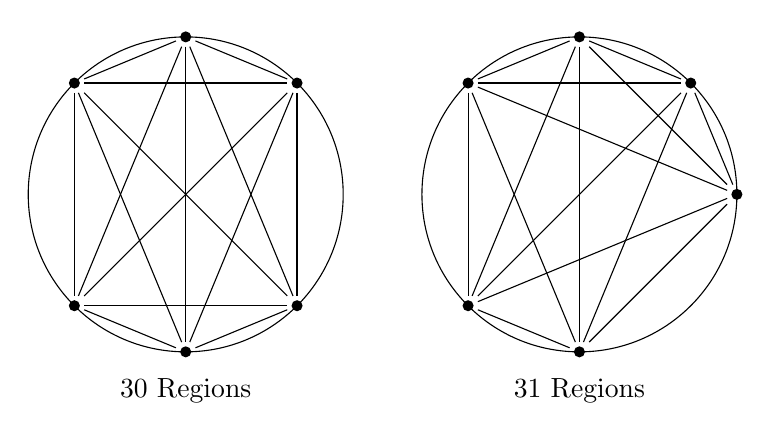
\begin{tikzpicture} % change these lines to a for-loop ?
\draw (0,0) circle[radius=2cm];
% top bot
\fill (0,2) circle[radius=2pt] node (t1) {};
\fill (0,-2) circle[radius=2pt] node (b1) {};
% left
\fill (-1.414,1.414) circle[radius=2pt] node (lt1) {};
\fill (-1.414,-1.414) circle[radius=2pt] node (lb1) {};
% right
\fill (1.414,1.414) circle[radius=2pt] node (rt1) {};
\fill (1.414,-1.414) circle[radius=2pt] node (rb1) {};
% lines
\draw (t1) -- (b1);
\draw (t1) -- (lt1);
\draw (t1) -- (lb1);
\draw (t1) -- (rt1);
\draw (t1) -- (rb1);
\draw (b1) -- (lt1);
\draw (b1) -- (lb1);
\draw (b1) -- (rt1);
\draw (b1) -- (rb1);
\draw (lt1) -- (lb1);
\draw (lt1) -- (rt1);
\draw (lt1) -- (rb1);
\draw (lb1) -- (rt1);
\draw (lb1) -- (rb1);
\draw (rt1) -- (rb1);
% regions
\draw (0,-2.5) node {30 Regions};

\draw (5,0) circle[radius=2cm];
% top bot
\fill (5,2) circle[radius=2pt] node (t2) {};
\fill (5,-2) circle[radius=2pt] node (b2) {};
% left
\fill (3.586,1.414) circle[radius=2pt] node (lt2) {};
\fill (3.586,-1.414) circle[radius=2pt] node (lb2) {};
% right
\fill (6.414,1.414) circle[radius=2pt] node (rt2) {};
\fill (7,0) circle[radius=2pt] node (rb2) {};
% lines
\draw (t2) -- (b2);
\draw (t2) -- (lt2);
\draw (t2) -- (lb2);
\draw (t2) -- (rt2);
\draw (t2) -- (rb2);
\draw (b2) -- (lt2);
\draw (b2) -- (lb2);
\draw (b2) -- (rt2);
\draw (b2) -- (rb2);
\draw (lt2) -- (lb2);
\draw (lt2) -- (rt2);
\draw (lt2) -- (rb2);
\draw (lb2) -- (rt2);
\draw (lb2) -- (rb2);
\draw (rt2) -- (rb2);
% regions
\draw (5,-2.5) node {31 Regions};
\end{tikzpicture}
\end{center}

Are you still not convinced that our formula is wrong? Try drawing a circle for \(n=7\) and \(n=8\), and compare your regions to your formula.

\section{Thinking Mathematically}

%Well, hopefully at the end of the course you will be able to answer this question for yourself.
Our goal is to teach you how to think mathematically. We want you to ask and answer questions based on logic. We want you to have sound reasoning. We want you to be able to back-up your answers with solid proof. We want your explanations to make sense, and we want to be convinced. In the real-world, no one is going to just \textit{accept} things you say unless you have good \textit{evidence} to back your claims. Our goal is to teach you how to (1) formally write your claims, and (2) provide proof for your claims. Mathematical thinking comes naturally for some, however for others it may take a whole semester. Keep working at it until you succeed.

\section{How to Succeed in this Course}

This course will provide you a toolkit of concepts from which you can pull to solve problems. Unlike methodological/algorithm-based courses (e.g.\ Calculus III), this course highly depends on your solid \textit{understanding} of the material. To succeed in this course, you will need to immerse yourself in the material. You will need to struggle through it until you understand. For some of you, this will be quick and easy. For others, not so much. That is okay. You will succeed so long as you put in the effort.

\section{Summary}

In order to succeed, you must:
\begin{itemize}
	\item Immerse yourself in the course content
	\item Struggle until you understand
	\item Think mathematically
\end{itemize}
\end{document}
